\section{Limiting Factors of the GPU}

In order to write code that is accelerated by the GPU, we must know which factors impact performance and to what extend. 
For this we have measured the performance of the following metrics: 

\begin{itemize}
    \item Allocating and freeing memory on the GPU.
    \item Copying memory to and from the GPU.
    \item Launching a kernel with increasing grid size.
\end{itemize}

To measure these metrics we have used our automated benchmarking tool. Each method was run with an exponentially scaling input to see how the performance of the operation scales. The code being measured can be seen in listings \ref{lst:cudaMalloc}, \ref{lst:cudaMemcopy} and \ref{lst:noop} in appendix A.

At the point of measuring these three metrics we had implemented matrix addition and multiplication. Crucially this meant we had only ever launched a single kernel to run our algorithm on the GPU and did not think to measure the cost of launching multiple kernels. This had major impact on the design of our QR-decomposition algorithm, which will be discussed later.\\

\noindent In the end we measured two more metrics, the code for which can be seen in listings \ref{lst:asynchronous kernels} and \ref{lst:synchronous kernels} in appendix A:

\begin{itemize}
    \item Launching kernels asynchronously.
    \item Launching kernels synchronously.
\end{itemize}

\subsection{Observations}

From our diagnostic benchmark (see figure \ref{fig:diagnostic_benchmark}) we can conclude the following:

\begin{itemize}
    \item The amount of blocks and threads spawned to execute a single kernel has no impact on performance.
    \item Allocating and freeing memory is done in constant yet significant amount of time. 
    \item Copying memory to and from the GPU takes an insignificant amount of time, until a massive amount of floats are being transferred. 
    \item Launching a kernel takes a significant amount of time.  
\end{itemize} 

\begin{figure}[ht]
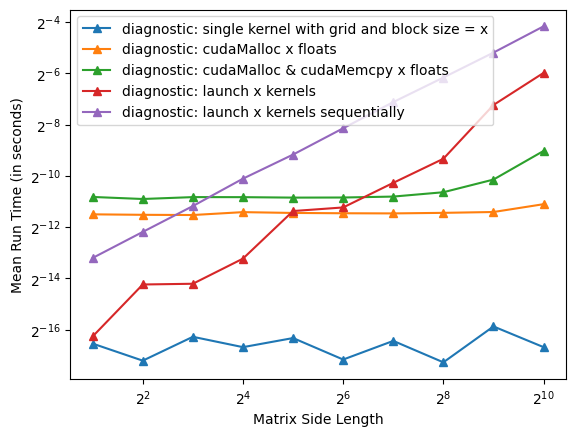
\includegraphics[width=\textwidth]{SavedBenchmarksAndDiagrams/Machine 2/Diagnostic/GPU Bench.png}
\caption{Diagram of benchmark analysis on GPU. $x$ is the matrix side length}
\label{fig:diagnostic_benchmark}
\end{figure}
